\documentclass[times,doublespace]{qjrms4}
\usepackage[colorlinks,bookmarksopen,bookmarksnumbered,citecolor=red,urlcolor=red]{hyperref}
\graphicspath{{/Users/ginochen/Gino/Paper/Paper_QJRMS/paper_final_revision}}
\begin{document}
	
%	\begin{figure*}[H]
%		\includegraphics[width=1\textwidth,height=0.6\textwidth]{autocorr_exp1n2.eps}
%		\caption{ \bf \label{autocorr}
%			n-lag autocorrelation coefficient $\gamma(n)$ of the $r^k$ time samples
%			in (a) $\tau_z=2$ and (b) $\tau_z=10$.\
%			}
%	\end{figure*}
%\clearpage
%	\begin{figure*}[H]
%		\includegraphics[width=1\textwidth, height=1\textwidth]{linearCurve_U_exp1n2_density.eps}
%		\caption{ \bf \label{linearCurve}
%			The $\bold{U^*}(X_1^k)$ samples (grey) in (a) $\tau_z=2$ and (b) $\tau_z=10$,
%%			A total of $320,000$ samples from $1600$ MTU sampled at every $0.005$ MTU.\
%			with density contours of the samples in (c) and (d), respectively.\
%			The fitted black curve is the deterministic parameterization $\bar{U}(X_1)$.\
%			}
%	\end{figure*}		
%\clearpage
%	\begin{figure*} [H]
%		\includegraphics[width=1\textwidth,height=0.6\textwidth]{linearCurve_pert_U_exp1n2.eps}
%		\caption{ \bf  \label{blackPertCurve}
%			The $\bold{U^*}(X_1^k)$ samples (grey), and the $U_p$ curves shifted from the deterministic curve $\bar{U}(X_1)$ (black)
%			in (a) $\tau_z=2$ and (b) $\tau_z=10$.\
%%			The plots are associated with 65 quadrature points.\
%%			65 black curves in each plot cover the entire $\bold{U^*}$ (grey circle).\
%			}
%	\end{figure*}
%
%\clearpage
%	\begin{figure*}[H]
%		\includegraphics[width=1\textwidth,height=0.6\textwidth]{hist_eU_2exp.eps}
%		\caption{ \bf  \label{hist_r}
%			The distribution of $e_{\text{clim}}$ in (a) $\tau_z=2$ and (b) $\tau_z=10$.\
%			}
%	\end{figure*}
%
%
%\clearpage
%	\begin{figure*} [H]
%		\includegraphics[width=1\textwidth,height=1\textwidth]{RMSEQpt_timeseries_300IC_meanao_exp1n2.eps} 
%		\caption{\bf \label{rmseQpt}
%			Time series of the RMSD between the exact solutions 
%			and the PCE approximations at $\tau_z=2$ (top) and $\tau_z=10$ (bottom).\ 
%			%on the quadrature points 
%			%averaged over 300 events at any given time.\ 
%			}
%	\end{figure*}
%\clearpage
%
%	\begin{figure*} [H]
%		\includegraphics[width=1\textwidth,height=1\textwidth]{respSfc_PClev8_MC1e3_exp1.eps} 
%		\caption{ \bf \label{respSfc1}
%			The evolution of the exact (grey) versus PCE-generated (black) 
%			ensemble model states ($X_1$ (top) and $Y_1$ (bottom)) as a function of 
%			the uniformly distributed $\xi$ in the standard domain $[-1 \ 1]$ at $\tau_z=2$.\
%%			$X_1$ (top) ordered from left to right as MTU = (3.5, 4.0, 4.5, 5.0, 5.5).\
%%			$Y_1$ (bottom) ordered as MTU = (5, 10, 15, 20, 25).\
%			}
%	\end{figure*}
%\clearpage
%
%	\begin{figure*} [H]
%		\includegraphics[width=1\textwidth,height=1\textwidth]{respSfc_PClev8_MC1e3_exp2.eps} 
%		\caption{ \bf \label{respSfc2}
%			As Figure {\ref{respSfc1}}, the exact (grey) versus PCE-generated (black) 
%			ensemble model states at $\tau_z=10$.\
%			}
%	\end{figure*}
%
%\clearpage
%	\begin{figure*} [H]
%		\includegraphics[width=1\textwidth,height=1\textwidth]{pdf_xa_xo_lev8_MC1e3_exp1.eps} 
%		\caption{ \bf \label{pdf1}
%			The evolution of the exact (grey) versus PCE-generated (black)
%			p.d.f. for the ensemble model states ($X_1$ (top) and $Y_1$ (bottom)) 
%			as a function of the uniformly distributed $\xi$ in the standard domain $[-1 \ 1]$ at $\tau_z=2$.\
%%			$X_1$ (top) ordered from left to right as MTU = (3.5, 4.0, 4.5, 5.0, 5.5).\
%%			$Y_1$ (bottom) ordered as MTU = (5, 10, 15, 20, 25).\
%			}
%	\end{figure*}
%
%\clearpage
%	\begin{figure*} [H]
%		\includegraphics[width=1\textwidth,height=1\textwidth]{pdf_xa_xo_lev8_MC1e3_exp2.eps} 
%		\caption{ \bf \label{pdf2}
%			As Figure {\ref{pdf1}}, the exact (grey) versus PCE-generated (black)  p.d.f. 
%			of the ensemble model states at $\tau_z=10$.\
%			}
%	\end{figure*}
%\clearpage
%
%	\begin{figure*} [H]
%		\includegraphics[width=1\textwidth,height=0.4\textwidth]{mev_mse_lev7_40pt_meanao.eps} 
%		\caption{\bf \label{mev_mse}
%			The evolution of MEV versus MSE
%			for the atmosphere (top) and ocean (bottom) components 
%			generated by perturbed parameter scheme (circle) and
%			additive stochastic parameterization (triangle) at $\tau_z=2$.\
%			}
%	\end{figure*}
%\clearpage
%
	\begin{figure*} [H]
		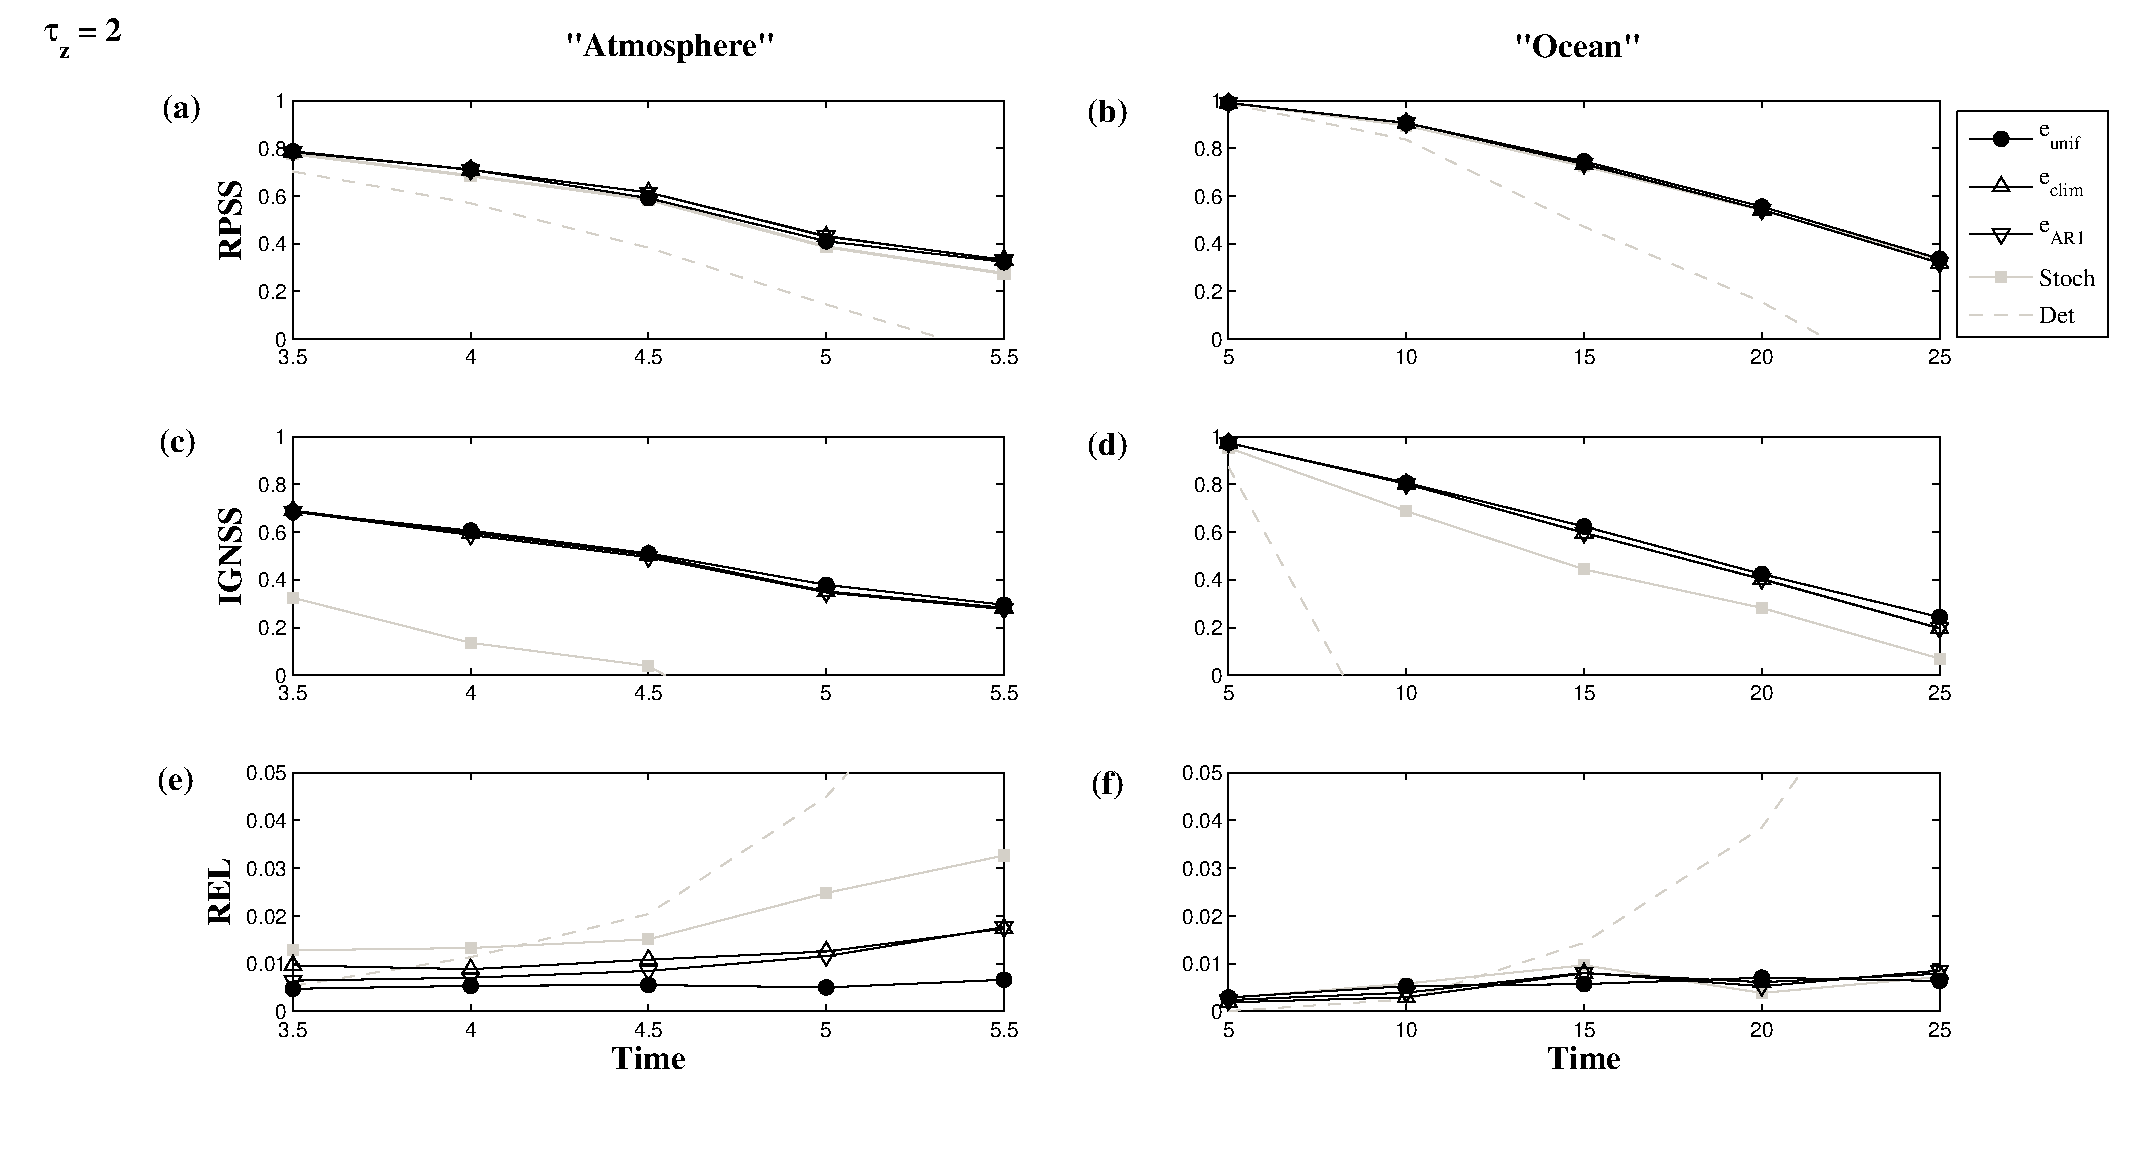
\includegraphics[width=1\textwidth,height=1\textwidth]{timeseries_alle_std00_lev8_40pt_meanao_exp1.eps}
		\caption{\bf \label{scoreTau2}
			Forecast scores RPSS (top), IGNSS (middle) and REL (bottom) for 
			the atmosphere (left) and ocean (right) components at $\tau_z=2$ generated by
			$e_{\text{unif}}$ (black circle), $e_{\text{clim}}$ (black upper triangle), $e_{\text{AR1}}$ (black lower triangle),
			\emph{Stoch} (grey square), and \emph{Det} (grey dashed-line).\
			The PCE approximated by $64^{\text{th}}$ degree polynomial.\
			}
	\end{figure*}	
%\clearpage
%
%	\begin{figure*} [H]
%		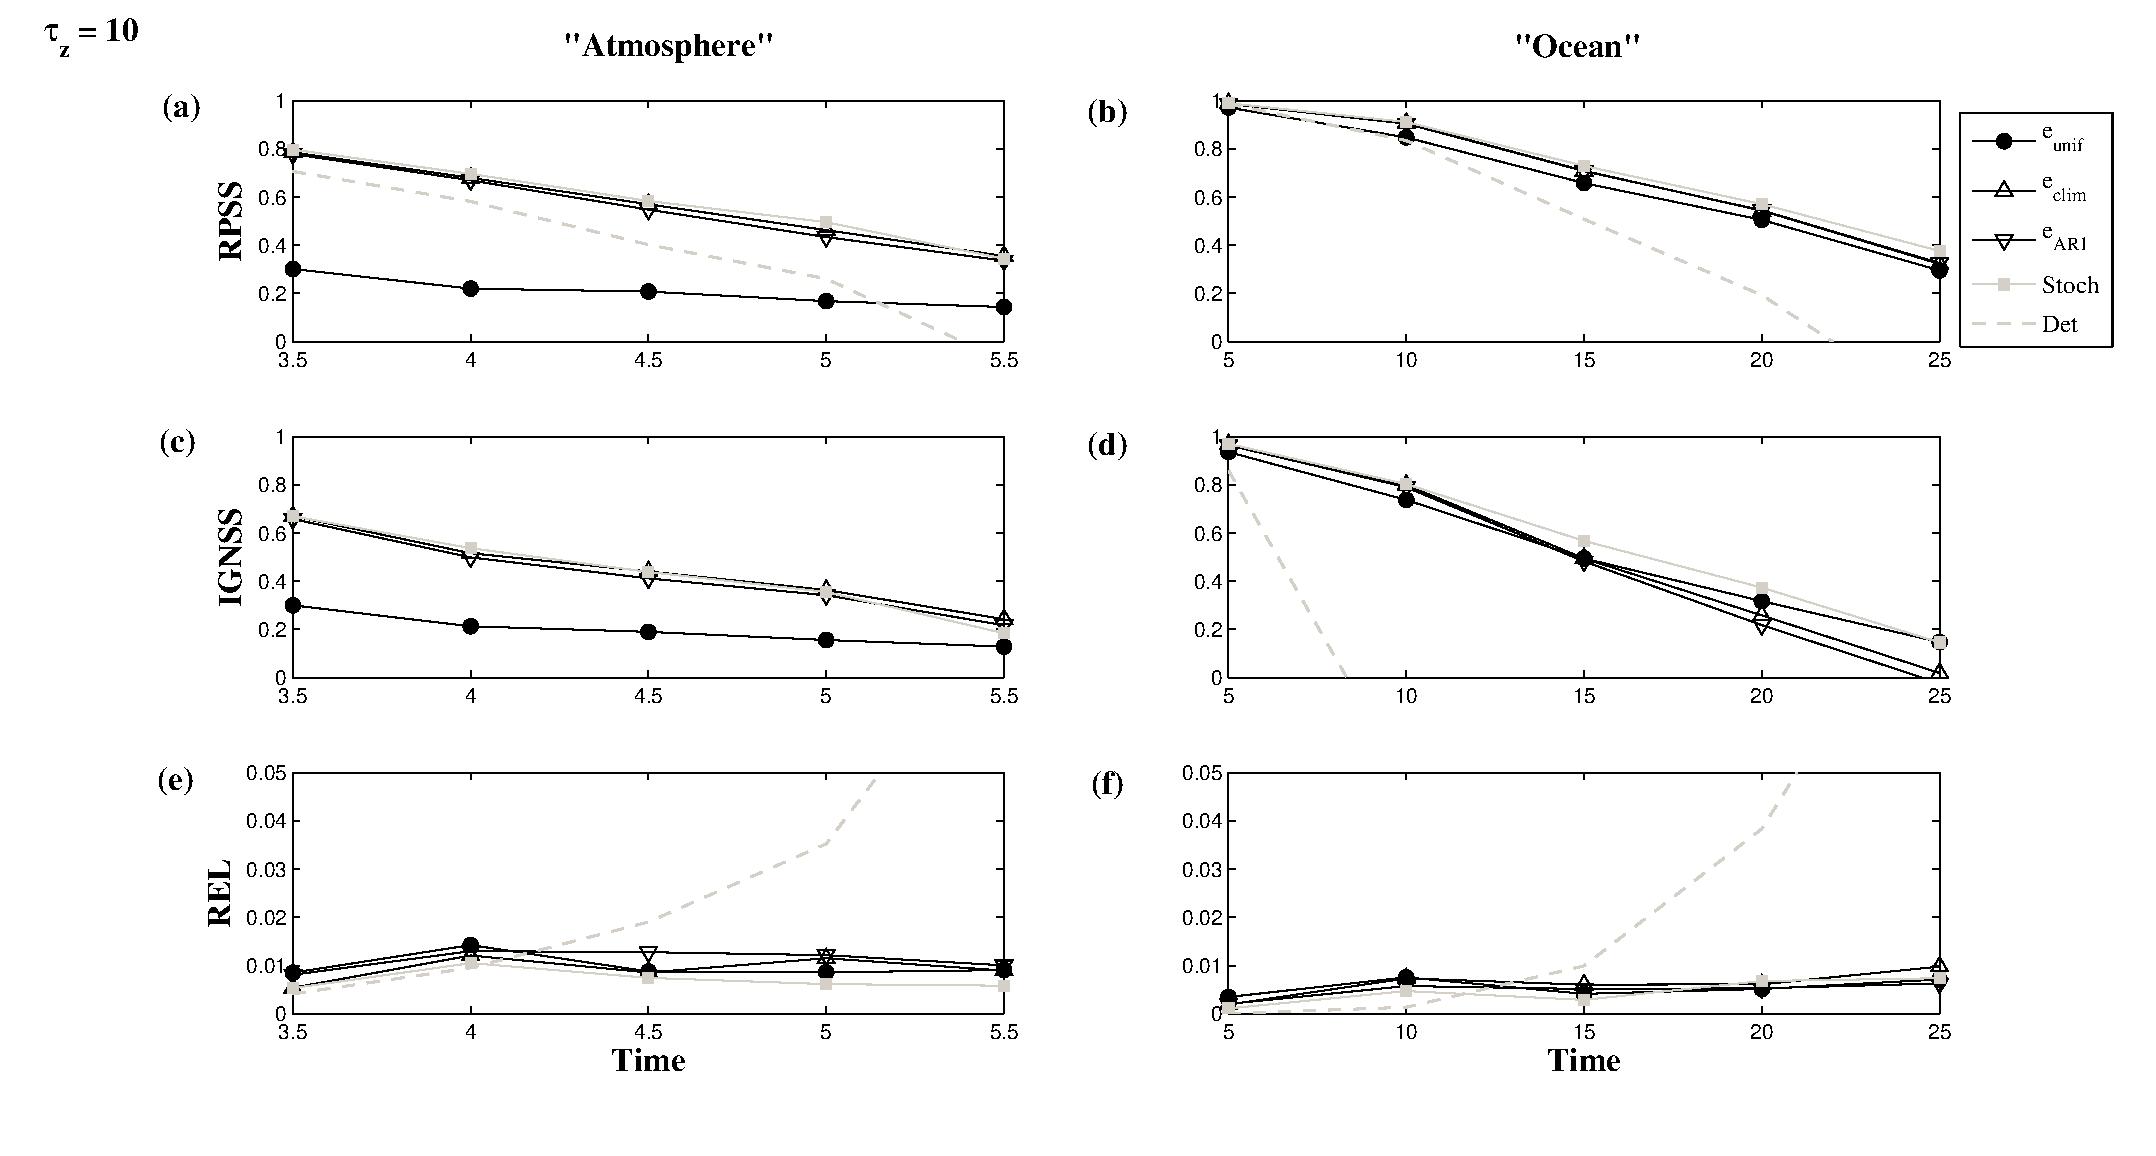
\includegraphics[width=1\textwidth,height=1\textwidth]{timeseries_alle_std00_lev8_40pt_meanao_exp2.eps}
%		\caption{\bf  \label{scoreTau10}
%			As Figure {\ref{scoreTau2}}, forecast scores RPSS, IGNSS and REL at $\tau_z=10$.\
%			}	
%	\end{figure*}
%\clearpage
%
%	\begin{figure*} [H]
%		\includegraphics[width=1\textwidth,height=1\textwidth] {timeseries_alle_std00_lev6_40pt_meanao_exp1.eps}
%		\caption{\bf \label{scoreTau2_lev6}
%			As Figure {\ref{scoreTau2}}, forecast scores RPSS, IGNSS and REL at $\tau_z=2$.\
%			The PCE approximated by $16^{\text{th}}$ degree polynomial.\
%			}
%	\end{figure*}	
	
\end{document}
